\documentclass[tikz,border=5pt]{standalone}
\usepackage{amsmath}
\usetikzlibrary{arrows.meta,calc}
\tikzset{vec/.style={-{Stealth[length=2.2mm]},thick},
dim/.style={thin},guide/.style={gray!65,dashed,thin},
chargePositive/.style={circle,draw=blue!70!black,fill=blue!12,inner sep=0pt,minimum size=6pt},
chargeNegative/.style={circle,draw=red!70!black,fill=red!12,inner sep=0pt,minimum size=6pt}}
\begin{document}
% statement-06: fixed x=-l,0,l; three separate vertical guides, not free motion.
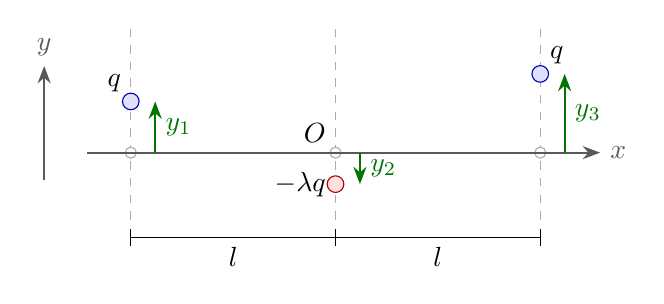
\begin{tikzpicture}
\foreach \x in {-2.6,0,2.6}
 {\draw[guide] (\x,-.85)--(\x,1.58);
  \draw[gray!65,fill=white] (\x,0) circle[radius=2pt];}
\draw[vec,black!65] (-3.15,0)--(3.36,0) node[right] {$x$};
\draw[vec,black!65] (-3.70,-.35)--(-3.70,1.10) node[above] {$y$};
\node[above left] at (0,0) {$O$};
\node[chargePositive] (P1) at (-2.6,.65) {};
\node[chargeNegative] (P2) at (0,-.40) {};
\node[chargePositive] (P3) at (2.6,1.0) {};
\node[above left] at (P1) {$q$};
\node[left] at (P2) {$-\lambda q$};
\node[above right] at (P3) {$q$};
\draw[vec,green!45!black] (-2.29,0)--(-2.29,.65) node[midway,right] {$y_1$};
\draw[vec,green!45!black] (.31,0)--(.31,-.40) node[midway,right] {$y_2$};
\draw[vec,green!45!black] (2.91,0)--(2.91,1.0) node[midway,right] {$y_3$};
\draw[dim] (-2.6,-1.08)--(0,-1.08)--(2.6,-1.08);
\foreach \x in {-2.6,0,2.6}{\draw[dim] (\x,-.97)--(\x,-1.19);}
\node[below] at (-1.3,-1.08) {$l$};
\node[below] at (1.3,-1.08) {$l$};
\end{tikzpicture}

% geometry-06: one generic pair; fixed horizontal h, actual distance r.
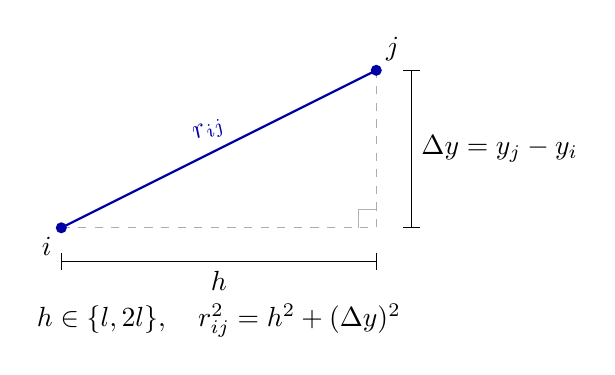
\begin{tikzpicture}
\coordinate (I) at (0,0); \coordinate (J) at (4,2); \coordinate (F) at (4,0);
\draw[guide] (I)--(F)--(J);
\draw[thick,blue!65!black] (I)--(J) node[midway,above,sloped] {$r_{ij}$};
\draw[gray!60] (3.77,0)--(3.77,.23)--(4,.23);
\fill[blue!65!black] (I) circle[radius=2pt] (J) circle[radius=2pt];
\node[below left] at (I) {$i$};\node[above right] at (J) {$j$};
\draw[dim] (0,-.43)--(4,-.43);
\draw[dim] (0,-.32)--(0,-.54) (4,-.32)--(4,-.54);
\node[below] at (2,-.43) {$h$};
\draw[dim] (4.45,0)--(4.45,2);
\draw[dim] (4.34,0)--(4.56,0) (4.34,2)--(4.56,2);
\node[right] at (4.45,1) {$\Delta y=y_j-y_i$};
\node at (2,-1.18) {$h\in\{l,2l\},\quad r_{ij}^2=h^2+(\Delta y)^2$};
\end{tikzpicture}

% modes-06: arrows are signed displacement ratios, NOT force arrows.
\begin{tikzpicture}
\foreach \panelShift/\modeName/\dispRatio in {0/Y/{1:1:1},3.8/\alpha/{1:0:-1},7.6/\beta/{1:-2:1}}
 {\begin{scope}[xshift=\panelShift cm]
  \draw[guide] (-.30,0)--(2.30,0);
  \node[chargePositive] at (0,0) {}; \node[chargeNegative] at (1,0) {}; \node[chargePositive] at (2,0) {};
  \node at (1,1.37) {$\modeName$};
  \node at (1,-2.16) {$\dispRatio$};
  \end{scope}}
\foreach \x in {0,1,2}{\draw[vec,gray!75] (\x,0)--(\x,.8);}
\draw[vec,blue!70!black] (3.8,0)--(3.8,.8);
\draw[vec,blue!70!black] (5.8,0)--(5.8,-.8);
\draw[vec,green!45!black] (7.6,0)--(7.6,.8);
\draw[vec,green!45!black] (8.6,0)--(8.6,-1.6);
\draw[vec,green!45!black] (9.6,0)--(9.6,.8);
\end{tikzpicture}

% stability-06: horizontal scale x=4 lambda, vertical omega^2/(c/m).
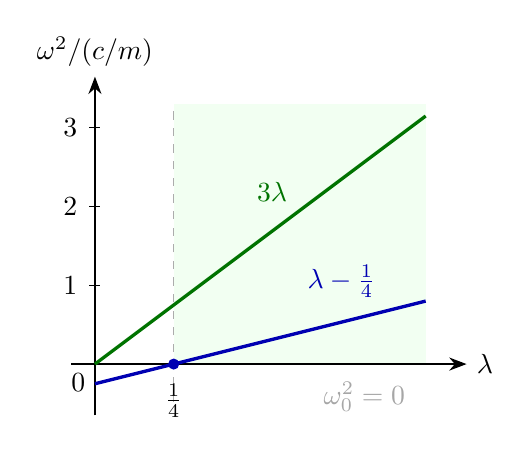
\begin{tikzpicture}
\fill[green!5] (1,0) rectangle (4.20,3.30);
\draw[vec] (-.30,0)--(4.72,0) node[right] {$\lambda$};
\draw[vec] (0,-.65)--(0,3.65) node[above] {$\omega^2/(c/m)$};
\draw[guide] (1,-.48)--(1,3.30);
\draw[blue!70!black,very thick] (0,-.25)--(4.20,.80);
\draw[green!45!black,very thick] (0,0)--(4.20,3.15);
\node[blue!70!black] at (3.13,1.05) {$\lambda-\frac14$};
\node[green!45!black] at (2.25,2.19) {$3\lambda$};
\fill[blue!70!black] (1,0) circle[radius=2pt];
\node[below] at (1,-.13) {$\frac14$};
\node[below left] at (0,0) {$0$};
\foreach \v in {1,2,3}
 {\draw[thin] (-.07,\v)--(.07,\v); \node[left] at (-.10,\v) {$\v$};}
\node[gray!70] at (3.42,-.42) {$\omega_0^2=0$};
\end{tikzpicture}

% chain-06: two sites per cell, a 2l period; nearest-neighbor separation l.
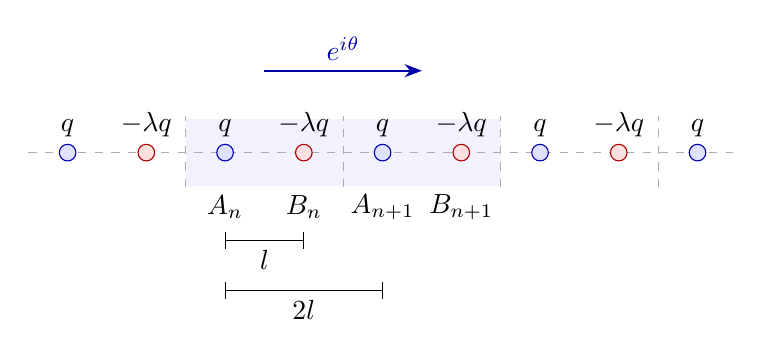
\begin{tikzpicture}
\fill[blue!5] (-.50,-.42) rectangle (1.50,.43);
\fill[blue!5] (1.50,-.42) rectangle (3.50,.43);
\draw[guide] (-2.5,0)--(6.45,0);
\foreach \x in {-2,0,2,4,6}
 {\node[chargePositive] at (\x,0) {}; \node[above] at (\x,.07) {$q$};}
\foreach \x in {-1,1,3,5}
 {\node[chargeNegative] at (\x,0) {}; \node[above] at (\x,.07) {$-\lambda q$};}
\foreach \x in {-.5,1.5,3.5,5.5}{\draw[guide] (\x,-.44)--(\x,.47);}
\node at (0,-.69) {$A_n$}; \node at (1,-.69) {$B_n$};
\node at (2,-.69) {$A_{n+1}$}; \node at (3,-.69) {$B_{n+1}$};
\draw[vec,blue!65!black] (.50,1.04)--(2.50,1.04) node[midway,above] {$e^{i\theta}$};
\draw[dim] (0,-1.12)--(1,-1.12);
\draw[dim] (0,-1.01)--(0,-1.23) (1,-1.01)--(1,-1.23);
\node[below] at (.50,-1.12) {$l$};
\draw[dim] (0,-1.75)--(2,-1.75);
\draw[dim] (0,-1.64)--(0,-1.86) (2,-1.64)--(2,-1.86);
\node[below] at (1,-1.75) {$2l$};
\end{tikzpicture}
\end{document}
